\documentclass{report}

\input{preamble}
\input{macros}
\input{letterfonts}

\title{\Huge{Math 120}}
\author{\huge{PSet 7}}
\date{Oct 24 2024}

\begin{document}

\maketitle
\newpage% or \cleardoublepage
% \pdfbookmark[<level>]{<title>}{<dest>}
\pdfbookmark[section]{\contentsname}{toc}
\tableofcontents
\pagebreak

\chapter{}
\section{PSet 7}

\qs{}{
    Calculate the given iterated integrals.
    \begin{enumerate}
        \item \( \int_0^1 \int_0^1 x \sqrt{1 + 4y} \, dy \, dx \)
        \item \( \int_0^1 \int_1^2 \frac{xe^x}{y} \, dy \, dx \)
    \end{enumerate}
}

\sol{
    \\
    1) 
    \[ \int_{0}^{1} \int_{0}^{1} x \sqrt{1 + 4y} \, dy \, dx \] 
    \[ \int_{0}^{1} x \sqrt{1 + 4y} \, dy \]
    \[ 1 + 4y = t \quad r = dt \]
    \[ x \int_{0}^{1} \frac{1}{4} \sqrt{t} dt \] 
    \[ \frac{1}{4}x \int_{0}^{1} \sqrt{t} dt \]  
    \[ \left. \frac{1}{4}x \cdot \frac{2t\sqrt{t}}{3} \right|_{0}^{1} \]
    \[ \left. \frac{1}{4}x \cdot \frac{2(1 + 4y)\sqrt{1+4y}}{3} \right|_{0}^{1} \]
    \[ \left. \frac{x\sqrt{1+4y}(1+4y)}{6} \right|_{0}^{1} \] 
    \[ \frac{x \sqrt{1+4}(1+4)}{6} - \frac{x\sqrt{1}{1}}{6} \] 
    \[ \frac{5x\sqrt{5}}{6} - \frac{x}{6} \] 
    \[ \int_{0}^{1} \frac{5x\sqrt{5}}{6} - \frac{x}{6} dx \] 
    \[ \frac{1}{6} \int_{0}^{1} 5\sqrt{5}x - x \, dx \] 
    \[ \frac{1}{6}\left(\int_{0}^{1} 5\sqrt{5} x dx - \int_{o}^{1} x \, dx \right)\]
    \[ \int_{0}^{1} 5 \sqrt{5}x \, dx \Rightarrow \left. \frac{5 \sqrt{5}x^{2}}{2} \right|_{0}^{1} \] 
    \[ \frac{5 \sqrt{5} (1)^{2}}{2} - 0  = \frac{5\sqrt{5}}{2} \] 
    \[ \int_{0}^{1} x \, dx \Rightarrow \left. \frac{x^{2}}{2} \right|_{0}^{1}\]  
    \[ \frac{1}{2} - 0 = \frac{1}{2}\] 
    \[ \frac{1}{6}\left( \frac{5\sqrt{5}}{2} - \frac{1}{2} \right) = \frac{5\sqrt{5} - 1}{12} \] 
    2) 
    \[ \int_{0}^{1} \int_{1}^{2}  \frac{xe^{x}}{y} \, dy \, dx \]
    \[ xe^{x} \int_{1}^{2} \frac{1}{y} \, dy \]
    \[ xe^{x} \left. \ln(y) \right|_{1}^{2} \Rightarrow xe^{x} \ln(2) - xe^{x}\ln(1) = xe^{x} \ln(2)\] 
    \[ \ln(2) \int_{0}^{1} xe^{x} \, dx  \]
    \[ \ln(2) \left. \left(xe^{x} -e^{x} \right) \right|_{0}^{1} \] 
    \[ \left(\ln(2)e - \ln(2)e \right) - \left(\ln(2)(0) - \ln(2)e^{0} \right) = 0 - (-\ln(2)(1)) = \ln(2) \]    
}

\qs{}{
    \begin{enumerate}
        \item[(a)] Sketch the solid whose volume is given by the iterated integral 
        \[ \int_0^1 \int_0^2 e^{-x^2 - y^2} \, dy \, dx. \]

        \item[(b)] Explain why 
        \[ \int_0^1 \int_0^2 e^{-x^2 - y^2} \, dy \, dx = \int_0^1 e^{-x^2} \, dx \cdot \int_0^2 e^{-y^2} \, dy. \]

        \item[(c)] Use Desmos to compute 
        \[ \int_0^1 \int_0^2 e^{-x^2 - y^2} \, dy \, dx. \]
        (Desmos will give a numerical approximation, but this is fine. In fact, there is no way to compute the antiderivatives necessary to get an exact answer.)
    \end{enumerate}
}

\sol{
    \begin{center}
        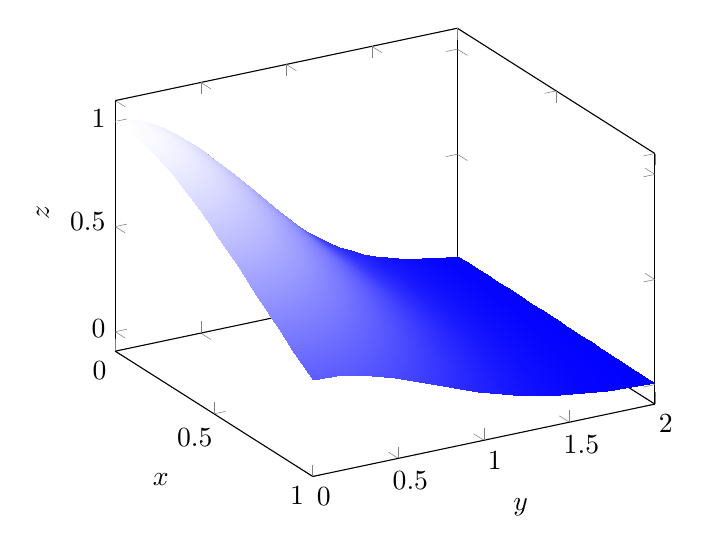
\begin{tikzpicture}
            \begin{axis}[
              view={60}{30}, 
              xlabel={$x$}, ylabel={$y$}, zlabel={$z$},
              domain=0:1, y domain=0:2,
              samples=30,
              colormap/viridis,
              mesh/interior colormap={bluewhite}{color=(blue) color=(white)},
              ]
              \addplot3[surf, shader=interp] 
              {exp(-x^2 - y^2)};
            \end{axis}
          \end{tikzpicture}       
    \end{center}
}

\qs{}{
    \begin{enumerate}
        \item[(a)] Find the average value of the function \( f(x, y) = \sin x \cos y \) on the rectangle \( R = [0, \pi] \times [-\pi/2, \pi/2]. \)
        
        \item[(b)] Use symmetry to find the average value of \( f(x, y) = \frac{4 \sin y}{e^{x^2}} - \frac{\cos x}{\ln y} + 3 \) on the region \( R = [2\pi, 4\pi] \times [2\pi, 6\pi]. \) Please explain your answer carefully.
    \end{enumerate}
}

\sol{
    a) 
    \[ f(x,y) = \sin x \cos y \]
    \[ R = [0, \pi ] \times [- \frac{\pi}{2}, \frac{\pi}{2}] \]
    \[ f_{avg} = \frac{1}{A(R)} \iint\limits_{R} f(x,y) dA \]
    \[ A(R) = (\pi - 0 ) \times (\frac{\pi}{2} - -\frac{\pi}{2}) = \pi^{2} \] 
    \[ \frac{1}{\pi^{2}} \int_{0}^{\pi} \int_{-\frac{\pi}{2}}^{\frac{\pi}{2}} \sin x \cos y  \, dy \, dx \] 
    \[ \sin x \int_{-\frac{\pi}{2}}^{\frac{\pi}{2}} \cos y \, dy \]
    \[ \left. (\sin x) \sin y \right|_{\frac{pi}{2}}^{\frac{\pi}{2}} \]  
    \[ (\sin x )\sin\left(\frac{\pi}{2}\right) - (\sin x )\sin\left(\frac{- \pi}{2}\right) = 2 \sin x \] 
    \[ \int_{0}^{\pi} 2 \sin x dx \]
    \[ \left. -2 \cos x \right|_{0}^{\pi} \]
    \[ -\cos \pi - (-2)\cos(0) = 4 \]
    \[ \frac{1}{\pi^{2}} \cdot 4 = \frac{4}{\pi^{2}} \]    
    b) 
    \[ f(x,y) = \frac{4 \sin y}{e^{x^{2}}} - \frac{\cos x}{\ln y} + 3 \]
    \[ R = [2 \pi, 4 \pi ] \times [2\pi, 6 \pi] \]
    \[ f_{avg} = \iint\limits_{R} f(x,y) dA \] 
    \[ A(R) = [4 \pi - 2 \pi ] \times [6\pi - 2 \pi] = 8 \pi^{2} \] 
    \[ \int_{2\pi}^{4 \pi} \int_{2 \pi}^{6 \pi} \frac{4 \sin y}{e^{x^{2}}} - \frac{\cos x}{\ln y }  + 3 \, dy \, dx \]
    \[ \iint\limits_{R} f(x,y) dA  - \iint\limits_{R} \frac{4 \sin y}{e^{x^{2}}} dA - \iint\limits_{R} \frac{\cos x}{\ln y } dA  + \iint\limits_{R} 3 dA\] 
    \[ \int_{2\pi}^{6 \pi} 4 \sin y \, dy = -4\left[ \cos y\right]_{2 \pi}^{6 \pi} = -4(6 \cos \pi - \cos 2 \pi) = -4(1 - 1) = 0 \]
    \[ \iint\limits_{R} f(x,y) \frac{4 \sin y}{e^{x^{2}}} dA = \int_{2 \pi}^{4 \pi} \frac{1}{e^{x^{2}}}dx \times 0 = 0 \]
    \[ \int_{2 \pi}^{4 \pi} {\cos x} dx = \left. \sin x \right|_{2 \pi}^{4 \pi} = sin 4 \pi - \sin 2 \pi = 0 - 0 = 0\] 
    \[ \iint\limits_{R} \frac{\cos x}{\ln y } dA = \int_{2 \pi}^{6 \pi} \frac{1}{\ln y} \times 0 = 0 \] 
    \[ \iint\limits_{R} 3 dA = 3 \times A(R) = 3 \times 8 \pi^{2} = 24 \pi^{2} \]
    \[ \frac{24 \pi^{2}}{8 \pi^{2}} = 3 \]  
}

\qs{}{
    In each part, draw the region \( D \), and evaluate the integral.
    \begin{enumerate}
        \item \( \iint_D \frac{y}{x^5 + 1} \, dA \), where \( D \) is the region \( D = \{(x, y) \mid 0 \leq x \leq 1, \, 0 \leq y \leq x^2 \}. \)
        \item \( \iint_D x^3 \, dA \), where \( D = \{(x, y) \mid 1 \leq x \leq e, \, 0 \leq y \leq \ln x \}. \)
    \end{enumerate}
}

\sol{
    1. 
    \[ \iint_D \frac{y}{x^5 + 1} \, dA  \quad D = \{(x, y) \mid 0 \leq x \leq 1, \, 0 \leq y \leq x^2 \} \]
    \[ \int_{0}^{1} \int_{0}^{x^{2}} \frac{y}{x^{5} + 1} \, dy \, dx \] 
    \[ \frac{1}{x^{5} + 1} \int_{0}^{x^{2}} y dy \]
    \[ \left. \frac{y^{2}}{2}\right|_{0}^{x^{2}} \Rightarrow \frac{\left(x^{2}\right)^{2}}{2} - \frac{0}{2} = \frac{x^{4}}{2} \]  
    \[ \int_{0}^{1} \frac{1}{x^{5} + 1} \times \frac{x^{4}}{2} dx \] 
    \[ x^{5} + 1 = t \quad dt = 5x^{4} dx \] 
    \[ \frac{1}{10} \int_{0}^{1} \frac{1}{t} dt \]
    \[ \left. \frac{1}{10} \ln|t| \right|_{0}^{1} \]
    \[ \left. \frac{1}{10} | x^{5} + 1 | \right|_{0}^{1} \]
    \[ \frac{1}{10} \ln(1^{5} + 1)   - \frac{1}{10}\ln(1) \]
    \[ \frac{1}{10} \ln(2) - \frac{1}{10} \ln(1) = \frac{1}{10} \ln(2) \]  
    2.    
    \[ \iint_D x^3 \, dA  \quad D = \{(x, y) \mid 1 \leq x \leq e, \, 0 \leq y \leq \ln x \} \]
    \[ \int_{1}^{e} \int_{0}^{\ln x} x^{3} \, dy \, dx \]  
    \[ x^{3} \int_{0}^{\ln x} 1 dy \]
    \[ \left. \left(x^{3}\right) y \right|_{0}^{\ln x} \]
    \[ x^{3} \ln x - 0 \]
    \[ uv - \int v \, du \] 
    \[ u = \ln x \quad du = \frac{1}{x}  \, dx \]
    \[ v = \frac{x^{4}}{4} \quad x^{3} dx \]   
    \[ \frac{\ln x \cdot x^{4}}{4} - \int \frac{x^{3}}{4} \, dx \]
    \[ \left[ \frac{\ln x^{4} \cdot x^{4}}{4} - \frac{x^{4}}{16}\right]_{1}^{e} \]
    \[ \left( \frac{\ln e \cdot e^{4} }{4} - \frac{e^{4}}{16} \right) - \left( \frac{\ln 1 \cdot 1^{4}}{4} - \frac{1^{4}}{16}\right)\] 
    \[ \left( \frac{\ln e \cdot e^{4} }{4} \right) - \left( 0 - \frac {1}{16} \right) \]
    \[ \left( \frac{e^{4}}{4} - \frac{e^{4}}{16}\right) + \frac{1}{16} \]   

}

\qs{}{
    Draw the region \( D \). Set up the iterated integrals for both orders of integration. 
    Then evaluate the double integral using the easier order and explain why it's easier.
    \[ \iint_D x^2 e^{-xy} \, dA \quad \text{where } D \text{ is bounded by } y = x, \, x = 4, \, \text{and } y = 0. \]
}

\sol{
    \[ \int_{0}^{4} \int_{0}^{x} x^{2}e^{-yx} \, dy \, dx \]
    \[ \int_{0}^{4} \int_{y}^{4} x^{2}e^{-yx} \, dx \, dy \]  
    \[ x^{2} \int_{y}^{4} e^{-yx} dy \] 
    \[ \left. \left( x^{2} \right) \frac{e^{-yx}}{x}  \right|_{0}^{x} \left(x^{2}\right) \frac{e^{-yx}}{x} - \left(x^{2} \right) \frac{e^{-0 \cdot x}}{x} \] 
    \[ xe^{-x^{2}} - x^{2}\cdot \frac{1}{x} \Rightarrow -xe^{-x^{2}} + x \]
    \[ \int_{0}^{4} -xe^{-x^{2}} + x \, dx  \Rightarrow \int_{0}^{4} -xe^{-x^{2}} \, dx \int_{0}^{4} x \, dx \]
    \[ -x^{2} = t \quad -2x = dt \]\
    \[ \int_{0}^{4} \frac{1}{2} e^{t} \, dt \Rightarrow \frac{1}{2} \int_{0}^{4} e^{t} \, dt \] 
    \[ \left. \frac{1}{2} e^{t} \right|_{0}^{4} \Rightarrow \left. \frac{1}{2} ^{x^{2}} \right|_{0}^{4} \] 
    \[ \frac{1}{2}e^{-4^{2}} - \frac{1}{2}e^{-0^{2}} \Rightarrow \frac{1}{2}e^{-16} - \frac{1}{2} \] 
    \[ \int_{0}^{4} x \, dx \]
    \[ \left. \frac{x^{2}}{2} \right|_{0}^{4} \] 
    \[ \frac{4^{2}}{2} - \frac{0^{2}}{2} = \frac{16}{2} = 8 \]
    \[ \int_{0}^{4} -xe^{-x^{2}} + x \, dx  = \frac{1}{2}e^{-16} + \frac{15}{2}\]      

}

\qs{}{
    \begin{enumerate}
        \item[(a)] Find the volume of the solid in the first octant enclosed by the parabolic cylinder \( y = 1 - x^2 \) and the planes \( z = 2 - y \) and \( z = y \).
        
        \item[(b)] Sketch the solid whose volume is given by the iterated integral 
        \[ \int_0^1 \int_0^{1-x} (2 - y^2) \, dy \, dx. \]
    \end{enumerate}
}

\sol{
    \[ y = - x^{2} \quad z = 2 - y \quad z = y \]
    \[ x,y,z \geq 0 \]
    \[ 2 - y = y \Rightarrow 2y = 2 \Rightarrow y = 1 \Rightarrow 0 \leq y \leq 1 - x^{2} \]
    \[ \text{height } = (2 -y) - y \Rightarrow 2 - 2y \]
    \[ V = \int_{0}^{1} \int_{0}^{1-x^{2}} 2 - 2y \, dy \, dx \]
    \[ \int_{0}^{1-x^{2}} 2 - 2y \, dy \]
    \[ \left. 2y - y^{2} \right|_{0}^{1-x^{2}} \]
    \[ 2\left(1-x^{2}\right) - \left(1-x^{2} \right) - 2(0) - (0)^{2} \] 
    \[ 2 - 2x^{2} - 1 + 2x^{2} - x^{4} \]
    \[ 1 - x^{4} \]
    \[ \int_{0}^{1} 1- x^{4} dx \]
    \[ \left. x - \frac{x^{5}}{5} \right|_{0}^{1} \]
    \[ 1 - \frac{1^{5}}{5} - 0 - \frac{0^{5}}{5} \]
    \[ 1 - \frac{1}{5} = \frac{4}{5} \]            
}

\qs{}{
    Sketch the region of integration and change the order of integration.
    \begin{enumerate}
        \item \( \int_0^1 \int_{4x}^4 f(x, y) \, dy \, dx \)
        \item \( \int_0^3 \int_{0}^{\sqrt{9 - y}} f(x, y) \, dx \, dy \)
        \item \( \int_0^4 \int_0^{\ln 2x} f(x, y) \, dy \, dx \)
    \end{enumerate}
}

\sol{\\
    a) 
    \[ \int_{0}^{1} \int_{4x}^{4} f(x,y) \, dy \, dx \]
    \[ \iint\limits_{D} f(x,y) dA \]
    \[ D = \{ (x,y)| 0 \leq x \leq 1, 4x \leq y \leq 4 \} \]
    \[ D = \{ (x,y) | 0 \leq y \leq 4 , 0 \leq x \leq \frac{1}{4} y \} \]\
    \[ \iint_{D} f(x,y) dA = \int_{0}^{4}\int_{0}^{\frac{1}{4}y} f(x,y) \, dx \, dy \]
    b)     
    \[ \int_{0}^{3} \int_{0}^{\sqrt{9-y}} f(x,y) \, dx \, dy \]  
    \[ \iint\limits_{D} f(x,y) dA \]
    \[ D = \{ (x,y)| 0 \leq x \leq \sqrt{9 - y}, 0 \leq y \leq 3 \} \]
    \[ x = \sqrt{9 -y} \quad x^{2} - 9 = - y \quad -x^{2} + 9 = y \]
    \[ -x^{2} + 9 = 3 \quad -x^{2} = - 6 \Rightarrow x^{2} = 6 \Rightarrow x = \sqrt{6} \]  
    \[ D = \{ (x,y)| 0 \leq y \leq -x^{2} + 9, \sqrt{6} \leq x \leq 3 \} \]
    \[ \int_{\sqrt{6}}^{3} \int_{0}^{-x^{2} + 9} f(x,y) \, dy \, dx  \]  
    c) 
    \[ \int_{0}^{4} \int_{0}^{ln 2x} \]
    \[ \iint\limits_{D} f(x,y) dA \quad D = \{ 0 \leq x \leq 4, 0 \leq y \leq ln x \} \]
    \[ y = ln 2x \Rightarrow y = ln 2(4) \Rightarrow y = ln 8 \Rightarrow 0 = ln 2x \Rightarrow ln 1 = \ln 2x 2x \Rightarrow x = \frac{1}{2} \] 
    \[ \iint\limits_{D} f(x,y) dA \quad D = \{ (x,y)| 0 \leq y \leq \ln 8 , \, \frac{1}{2} \leq x \leq \frac{e^{y}}{2} \} \]
    \[ \int_{0}^{\ln 8 } \int_{\frac{1}{2}}^{\frac{e^{y}}{2}}f(x,y) \, dx \, dy \]      
}

\qs{}{
    Evaluate the integral 
    \[ \int_0^1 \int_x^1 e^\frac{x}{y} \, dy \, dx \]
    by reversing the order of integration.
}

\sol{
    \[ \] 
}

\qs{}{
    Evaluate the given integral by converting to polar coordinates. Be sure to draw the region of integration in each part.
    \begin{enumerate}
        \item \( \iint_R (x + y) \, dA \), where \( R \) is the region that lies to the left of the \( y \)-axis between the circles \( x^2 + y^2 = 1 \) and \( x^2 + y^2 = 4 \).
        \item \( \iint_R y e^x \, dA \), where \( R \) is the region in the first quadrant enclosed by the circle \( x^2 + y^2 = 25 \).
    \end{enumerate}
}

\sol{
    a) 
    \[ x \leq 0 \quad x + y^{2} = 1 \quad x^{2} + y^{2} = 4 \]
    \[ x = r \cos \theta \quad y = r \sin \theta \quad dA = r dr \, d \theta \]
    \[ R: 1 \leq r \leq 2 \]
    \[ x + y = r \cos \theta + r \sin \theta \Rightarrow r ( \cos \theta \sin \theta ) \]
    \[ \int_{\frac{\pi}{2}}^{\frac{\pi}{2}} \int_{1}^{2} r(\cos \theta \sin \theta ) r \, dr \, d\theta\] 
    \[ \cos \theta + \sin \theta \int_{1}^{2} r^{2} dr \]
    \[ \left. \frac{r^{3}}{3} \right|_{1}^{2} \]
    \[ \frac{2^{3}}{3} - \frac{1}{3} =  \frac{7}{3} \]
    \[ \frac{7}{3} \int_{\frac{\pi}{2}}^{\frac{3 \pi}{2}} \cos \theta + \sin \theta \, d \theta \]
    \[ \left. \frac{7}{3} \sin \theta \right|_{\frac{\pi}{2}}^{\frac{3 \pi}{2}} - \left. \frac{7}{3} \cos \theta \right|_{\frac{\pi}{2}}^{\frac{3 \pi }{2}} \]   
    \[ \frac{7}{3}(-1) - \frac{7}{3}(1) = -\frac{14}{3} \]
    \[ -\frac{7}{3} \cos \frac{3 \pi}{2} + \frac{7}{3} \cos \frac{\pi}{2} \]
    \[ - \frac{7}{3} (0) + \frac{7}{3} = 0 \]
    \[ - \frac{14}{2}\]
    b)           
    \[ \iint\limits_{R} ye^{x} dA \]
    \[ x = r \cos \theta \quad y = r \sin theta \quad x^{2} + y^{2} = 25 \]
    \[ \text{ 1st quadrant } \quad 0 \leq \theta \leq \frac{\pi}{2} \]
    \[ ye^{x} \Rightarrow r \sin \theta e ^{r \cos \theta } \]
    \[ dA = r \, dr \, d\theta \]
    \[ \int_{0}^{\frac{\pi}{2}} \int_{0}^{5} r \sin \theta e^{r \cos \theta }\] 
    \[  I(\theta) = \int_{0}^{5} r^{2} \sin \theta \, e^{r \cos \theta} \, dr \] 
    \[ \frac{\partial}{\partial \theta} e^{r \cos \theta} = -r \sin \theta \, e^{r \cos \theta} \]
    \[ r \sin \theta e^{r \cos \theta} = - \frac{\partial}{\partial \theta} e^{r \cos \theta} \]
    \[ I = \int_{0}^{\frac{\pi}{2}} \int_{0}^{5} - r \frac{\partial}{\partial \theta} e^{r \cos \theta} \, dr \, d\theta \]
    \[ I = - \int_{0}^{5} r \left( \int_{0}^{\frac{\pi}{2}} \frac{\partial }{\partial \theta} e^{r \cos \theta} \, d\theta \right) dr \]
    \[ \int_{0}^{\frac{\pi}{2}} \frac{\partial}{\partial \theta} e^{r \cos } \, d \theta = \left. e^{r \cos \frac{\pi}{2}} \right|_{0}^{\frac{\pi}{2}} \] 
    \[ e^{r \cos \frac{\pi}{2}} - e^{r \cos \theta} = e^{r \cdot 0} - e^{r \cdot 1} = 1 - e^{r} \] 
    \[ I = \int_{0}^{5} re^{r} dr - \int_{0}^{3} r dr \]
    \[ u = r \quad du = dr \quad v = e^{r} \quad dv = e^{r} dr \]
    \[ \int_{0}^{5} re^{r} dr = re^{r} - \int_{0}^{5} e^{r} dr = re^{r} -e^{r} + K \]
    \[ \int_{0}^{5} re^{r} dr = \left[ re^{r} - e^{r} \right]_{0}^{5} = \left( 5e^{5} - e^{5} \right) - (0 - e^{0}) = 4e^{5} + 1 \]
    \[ \int_{0}^{5} r dr = \left. \frac{1}{2}r^{2} \right|_{0}^{5} = \frac{1}{2} (25 - 0 ) = \frac{25}{2} \] \
    \[ I = (4e^{5} + 1) - \frac{25}{2} = 4e^{5} - 11.5  \]              
}

\qs{}{
    Use polar coordinates to find the volume of the given solid.
    \begin{enumerate}
        \item[(a)] Inside the sphere \( x^2 + y^2 + z^2 = 4 \) and outside the cylinder \( x^2 + y^2 = 1 \).
        \item[(b)] Bounded by the paraboloids \( z = 3x^2 + 3y^2 \) and \( z = 4 - x^2 - y^2 \).
    \end{enumerate}
}

\sol{
    a) 
    \[ x^{2} + y^{2} + z^{2} = 4 \quad  x^{2} + y^{1} = 1  \] 
    \[ x = r \cos \theta \quad y = r \sin \theta \quad 0 \leq \theta \leq 2 \pi \]
    \[ r^{2} + z^{2} = 4 \quad x^{2} + y^{2} = 1 \Rightarrow r^{2} = 1 \Rightarrow r = 1 \]
    \[ r^{2} + z^{2} = 4 \Rightarrow r^{2} = 4 - z^{2} \Rightarrow r = \sqrt{4 - z^{2}} \]
    \[ V = \iint\limits_{D} \left[ z_{\text{upper}} - z_{\text{lower}} \right]\]
    \[ V = \int_{0}^{2\pi}\int_{1}^{2}   r \sqrt{4 - r^{2} - \left( - \sqrt{4 - r^{2}} \right)}  r \, dr \, d \theta \]
    \[ V = 2 \int_{0}^{2 \pi} \int_{1}^{2} \sqrt{4 - r^{2}} \, dr \, d \theta \]
    \[ 4 - r^{2} = t \quad -2r = dt \]
    \[ - \int_{1}^{2} \frac{1}{2} \sqrt{t} dt \Rightarrow - \frac{1}{2} \int_{1}^{2} \sqrt{t} dt = \left. - \frac{1}{2} \cdot \frac{2t\sqrt{t}}{3} \right|_{1}^{2} \]
    \[ \left. - \frac{1}{2} \cdot \frac{2(4-r^{2})\sqrt{4-r^{2}}}{3} \right|_{1}^{2} \left( - \frac{1}{2} \cdot \frac{2(4-2^{2})\sqrt{4-2^{2}}}{3} \right) - \left( - \frac{1}{2} \cdot \frac{2(4-1^{2})\sqrt{4-1^{2}}}{3}\right) \]    
    \[ V = 2 \left( \int_{2}^{2\pi} d \theta \right) \left(\int_{1}^{2} r\sqrt{4-r^{2}} dr \right)\]   
    \[ \int_{0}^{2 \pi} d \theta = 2 \pi \quad V = 2 \cdot 2 \pi \cdot \int_{1}^{2} r \sqrt{4-r^{2}} dr = 4 \pi \int_{1}^{2} r \sqrt{4 - r^{2}} dr \]
    \[ - \left(- \frac{1}{2} \cdot \frac{2(3)\sqrt{3}}{3} \right) \Rightarrow \left( \frac{1}{2} \sqrt{3} \right)  \Rightarrow - (- \sqrt{3}) \]
    \[ 4 \pi \sqrt{3} \]  
    b) 
    \[ z = 3x^{2} 3y^{2} = 3\left(x^{2} + y^{2} \right) = 3\left(x^{2} + y^{2}\right) = 3r^{2} \]
    \[ z = 4 - x^{2} - y^{2} = 4 - r^{2} \]
    \[ 3r^{2} = 4 - r^{2} \]
    \[ 4r^{2} = 4 \Rightarrow r = 1 \]
    \[ \int_{0}^{2\pi} \int_{0}^{1} \left( 4 - r^{2} - 3r^{2} \right)r \, dr \, d\theta \]
    \[ \int_{0}^{2\pi} \int_{0}^{1} \left( 4 - 4r^2\right)r \, dr \, d\theta \]
    \[ \left.  2r - r^{4}\right|_{0}^{1} \, d \theta \Rightarrow \left(2(1)^{2} - 1 \right) - 0 \]
    \[ \int_{0}^{2 \pi} 1 \, d\theta \] 
    \[ \left. \theta \right|_{0}^{2\pi} = 2\pi \]             
}

\qs{}{
    Evaluate the iterated integral 
    \[ \int_0^b \int_{-\sqrt{b^2 - y^2}}^0 x^2 y \, dx \, dy \]
    by converting to polar coordinates.
}

\sol{   
    \[ \int_{0}^{b} \int_{- \sqrt{b^{2} - y^{2}}}^{0} x^{2}y \, dx \, dy\]
    \[ y = 0 \quad \text{to } \quad y = b \] 
    \[ x = - \sqrt{b^{2} - y^{2} } \text{to } \quad \text{to } {x = 0 } \]
    \[ \text{left half of } x^{2}+y^{2} = b^{2} \]
    \[ x = r \cos \theta \quad y = r \sin \theta \quad 0 \leq r \leq b \quad \frac{\pi}{2} \leq \theta \pi \] 
    \[ x^{y} = (r \cos \theta )^{2} (r \sin \theta) = r^{3} \cos \theta \sin \theta \]
    \[ \int_{\frac{\pi}{2}}^{\pi} \int_{0}^{b} \left(r^{3} \cos^{2} \theta \sin \theta \right) r \, dr \, d\theta \]
    \[ \int_{\frac{\pi}{2}}^{\pi} \int_{0}^{b} r^{4} \cos^{2} \theta \sin \theta \, d\theta \, dr \]
    \[ \cos^{2}\theta \sin \theta \int_{0}^{b} r^{4} \, dr \] 
    \[ \left. \cos^{2}\theta \sin \theta \frac{r^{5}}{5} \right|_{0}^{b} \]
    \[ \cos^{2}\theta \sin \theta \frac{b^{5}}{5} - 0 \]     
    \[ \int_{\frac{\pi}{2}}^{\pi} \frac{b^{5}}{5} \cos^{2}\sin \theta \, d \theta \]
    \[ \frac{b^{5}}{5} int_{\frac{\pi}{2}}^{\pi} \cos^{2}\sin\theta \]
    \[ \left. \frac{b^{5}}{5} \frac{\cos^{3}\theta}{3} \right|_{\frac{\pi}{2}}^{\pi} \]
    \[ \left(\frac{b^{5}}{5}\right)\left(\frac{\cos^{3} \frac{\pi}{2}}{3}\right) - \left(\frac{b^{5}}{5}\right)\left(\frac{\cos^{3} \pi }{3}\right)\] 
    \[ 0 - \frac{b^{5}}{5} \cdot \frac{-1}{3} \]
    \[ \frac{b^{5}}{15}\]        
}

\qs{}{
    Let \( D \) be the disk with center at the origin and radius \( a \).
    \begin{enumerate}
        \item[(a)] Use your intuition: what do you expect is the average distance from points on the disk to the origin?
        \begin{itemize}
            \item less than \( a/2 \)
            \item \( a/2 \)
            \item between \( a/2 \) and \( a \)
            \item more than \( a \)
        \end{itemize}
        Give an intuitive explanation of your answer.

        \item[(b)] What is the average distance from points in the disk to the origin?
    \end{enumerate}
}

\sol{
    The area of the disk should be greater on the interval of $\left[ \frac{a}{2}, a \right] $ than from $\left[0, \frac{a}{2} \right]$ which means 
    there are more points on the interval of  $\left[ \frac{a}{2}, a \right] $ meaning hte average distance is on this interval. 
    \\
    b) \\
    \[ D = \frac{1}{A} \iint\limits_{A} d \, \, da \]
    \[ D = \frac{1}{A} \int_{0}^{2\pi}\int_{0}^{a} r \cdot r \, dr \, d\theta \]
    \[ \left. \frac{r^{3}}{3}\right|_{0}^{a} \Rightarrow \frac{a^{3}}{3} - 0  = \frac{a^{3}}{3} \]
    \[ A = a^{2}\pi \]
    \[ \frac{1}{a^{2} \pi} \int_{0}^{2\pi} \frac{a^{3}}{3} \, d\theta \]
    \[ \left. \frac{1}{a^{2} \pi} \left(\frac{a^{3}}{3}\right) \right|_{0}^{2\pi} \]
    \[ \frac{2a}{3} \]       
}

\end{document}
